\chapter{Technology Review}

\section{Executive Dashboard}
When it came to developing the Executive Dashboard for data analysis it was crucial to select the tools that could transform data into easily comprehensible information. After conducting research and exploring alternatives Angular and Chart.js were chosen for specific reasons.

\subsection{Angular}
Angular is based on TypeScript and is an open-source framework, and it's a great tool for building client-side web applications. It can be used for single-page applications (SPAs) or for enterprise-level solutions. 

\subsubsection{Main Concepts: Components, Modules and Services}
Angular is composed of three foundational blocks: Components, Modules and services.

\subsubsection{Components} Components are like Lego blocks of the application. Each component holds a portion of the user interface and its behaviour. Components serve as the bridge between the application data and what the user experiences on the screen.\cite{angular-components}

\subsubsection{Modules} In Angular modules serve as containers that group related components, directives, and services together that can be combined with other modules. It plays an important role in improving maintainability and re-usability, key concepts of Angular development.\cite{angular-modules}

\subsubsection{Services} Angular services use typescript classes with injectable decorators. The decorator tells angular that the class is a service and can be injected into other components that need that service.\cite{angular-services}


\subsection{Angular architecture}
Angular uses the Model-View-Controller (MVC) pattern, with a variation known as Model-View-ViewModel (MVVM). The controller is responsible for the interaction between the model and the view.

\begin{figure}[ht]
    \centering
    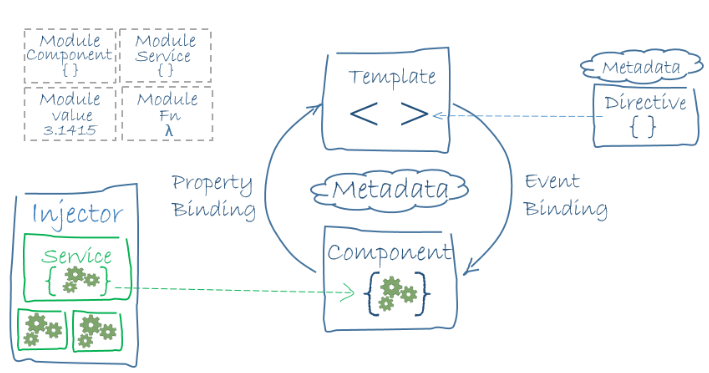
\includegraphics[width=0.85\linewidth]{images/angular-arch.png} 
    \caption{Angular application architecture}
    \label{fig:angular-arch}
\end{figure}

\subsection{Advantages of using Angular}
\subsubsection{Component-Based Architecture} 
 As mentioned earlier in discussions Angular organisess its functionalities into components. These components have the ability to communicate with each other enabling updates to sections without affecting the rest of the application.

\subsubsection{Mobile-Friendly Approach} 
Angular incorporates techniques such, as lazy-loading, which means loading parts of the application (like images) only when they are needed. This ensures that users do not experience long waiting times.

\subsubsection{Two-Way Data Binding} 
With Angular two way data binding data can seamlessly flow between the component and the view allowing for synchronization.

\subsubsection{Asynchronous Programming} 
By utilizing programming executes code in a non-sequential manner and employs multi-threading to enhance performance. This speeds up operations and prevents system freezes, providing users with a seamless experience.
 
\subsubsection{Single-Page Applications}
Angular creates a dynamic single-page application which can be navigated without page reloads, improving the user experience with better user interaction and engagement.

\subsubsection {Code Re-usability} 
The component-based architecture of Angular promotes the re-usability of UI components saving development time.

\subsubsection{Dependency Injection} 
With dependency injection in place, Angular allows for the creation of objects that rely on other objects. This improves modularity and efficiency, within the app.

\subsubsection{Angular Material} 
Angular's documentation offers a range of built user interface components and modules that adhere to Google's Material Design principles. This greatly facilitates the developer's work, simplifying the design process and enabling application development.

\subsubsection{Angular CLI} Angular command line interface gives the developer the ability to generate Angular projects, modules, services, and components with a single command, this not only saves time but also reduces configuration errors, it gives the developer the freedom to dive into creative aspects of the project, focusing on innovation and functionality rather than getting bogged down by initial setup complexities.